\documentclass[tikz, border=5px]{standalone}
\definecolor{w}{RGB}{255,255,255}
\begin{document}
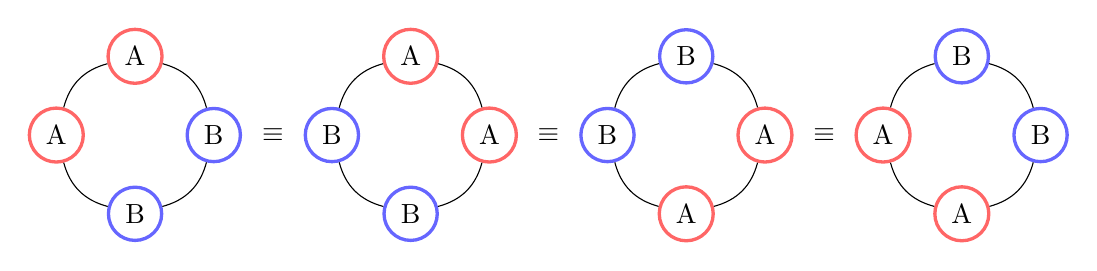
\begin{tikzpicture}[
        red/.style={circle, draw=red!60, fill=w, very thick},
        blue/.style={circle, draw=blue!60, fill=w, very thick},
        green/.style={circle, draw=green!60,  fill=w, very thick},
    ]

    \node[red] (1) at (0,0) {A};
    \node[red] (2) at (1,1) {A};
    \node[blue] (3) at (2,0) {B};
    \node[blue] (4) at (1,-1) {B};

    \path
    (1) edge[bend left, looseness=1] (2)
    (2) edge[bend left, looseness=1] (3)
    (3) edge[bend left, looseness=1] (4)
    (4) edge[bend left, looseness=1] (1)
    ;

    \node at (2.75,0) {$\equiv$};

    \node[blue] (5) at (3.5,0) {B};
    \node[red] (6) at (4.5,1) {A};
    \node[red] (7) at (5.5,0) {A};
    \node[blue] (8) at (4.5,-1) {B};

    \path
    (5) edge[bend left, looseness=1] (6)
    (6) edge[bend left, looseness=1] (7)
    (7) edge[bend left, looseness=1] (8)
    (8) edge[bend left, looseness=1] (5)
    ;


    \node at (6.25,0) {$\equiv$};

    \node[blue] (9) at (7,0) {B};
    \node[blue] (10) at (8,1) {B};
    \node[red] (11) at (9,0) {A};
    \node[red] (12) at (8,-1) {A};

    \path
    (9) edge[bend left, looseness=1] (10)
    (10) edge[bend left, looseness=1] (11)
    (11) edge[bend left, looseness=1] (12)
    (12) edge[bend left, looseness=1] (9)
    ;


    \node at (9.75,0) {$\equiv$};

    \node[red] (13) at (10.5,0) {A};
    \node[blue] (14) at (11.5,1) {B};
    \node[blue] (15) at (12.5,0) {B};
    \node[red] (16) at (11.5,-1) {A};

    \path
    (13) edge[bend left, looseness=1] (14)
    (14) edge[bend left, looseness=1] (15)
    (15) edge[bend left, looseness=1] (16)
    (16) edge[bend left, looseness=1] (13)
    ;
\end{tikzpicture}

\end{document}